\documentclass{beamer}

\usepackage[utf8]{inputenc}
\usepackage{graphicx}
\usepackage{xcolor}

\graphicspath{{img}}
\definecolor{azul marino}{RGB}{60,220,150}


\setbeamercolor{background canvas}{bg = azul marino}


\title{Presentación Moogle!}
\author{David Michel García Batista}
\date{Julio de 2023}
\usetheme{CambridgeUS}

\begin{document}
\maketitle
\begin{frame}{Moogle! ¿En qué consiste esta herramienta?}
    La aplicación web Moogle! es un modelo de búsqueda que nos devolverá los documentos más 
    relevantes y similares a la información que ingrese su usuario en lo que denominaremos \textbf{Query}.
\begin{center}
    
\includegraphics[scale=0.35]{moogle-1.png}
\end{center}
\tiny\textbf{El nombre de este programa es netamente original. Cualquier parecido con otro programa o aplicación de la vida real es pura coincidencia}    
\end{frame}

\begin{frame}
\frametitle{¿Cómo funciona?}
\large{\textbf{Nuestra problemática es simple, solucionarla no tanto}}\\
Tenemos una serie de documentos .txt y en dependencia de una Query ingresada por el usuario debemos devolver los más relevantes\\
¿Qué hacer entonces?\\
\begin{center}

\includegraphics[scale=0.6]{hombre duda.png}
\end{center}
\end{frame}

\begin{frame}
    \frametitle{¡Pues claro!}
    \large{Cómo buenos matemáticos que somos, calcularemos la \textbf{relevancia} de cada documento con respecto a la Query para compararlos y así determinar aquellos documentos más importantes.
    Él metodo será utilizando el TF-IDF (Ver fig 1 Anexos) y la similitud de cosenos}
\end{frame}

\begin{frame}
    \frametitle{De qué va la cosa:}
    Nuestro programa funcionará con varias clases encaminadas a cada función que se necesitará para resolver nuestra problemática:
    \begin{enumerate}
        \item Recibir el contenido de los documentos y procesarlos para poder trabajar 
        \item Calcular la importancia de estos documentos y de la Query ingresada
        \item Crear una base de datos que almacene toda esta información y permita compararla y maniobrarla
    \end{enumerate}
    Y pues como tenemos 3 funciones, se designará una clase a cada una de ellas.
\end{frame}

\begin{frame}
    \frametitle{Clase Document}
    Será quien realizará el trabajo inicial, se llenará las manos de información y procesará cada texto
    \begin{itemize}
        \item Buscar (Directory.GetCurrentDirectory)
        \item Recopilar información (Directory.GetFiles)
        \item Fragmentar textos (Método Split Text)
        \item Extraer Títulos (Método Get Title)
    \end{itemize}
    A eso se dedica, de eso vive, ese es su propósito...\\
    \small{\textbf{Un poco triste no creen?}}
\end{frame}

\begin{frame}
    \frametitle{Clase TF-IDF}
    \large{Será quien haga el trabajo sucio del proyecto. Números van y números vienen}\\
    Calcular el TF-IDF (Term Frequency-Inverse Document Frequency) de cada palabra. Una vez obtenidos se puede hallar la relevancia  con la Query mediante la similitud de cosenos\\
    (Ver fig 2 y 3 Anexos)
\end{frame}

\begin{frame}
    \frametitle{Clase Database}
    Debido a que la originalidad es nuestra principal característica, esta clase como su nombre indica será quien creará una base de datos para organizar la información\\
    Se utilizarán dos componentes:
    \begin{enumerate}
        \item Diccionarios
        \item Listas
    \end{enumerate}
    Con ellas se agruparán todos los documentos con cada palabra y su TF-IDF asociado así como la Query para determinar las relevancias y comparando para finalmente devolver los resultados.
\end{frame}

\begin{frame}
    \frametitle{Anexos}
    \begin{center}
    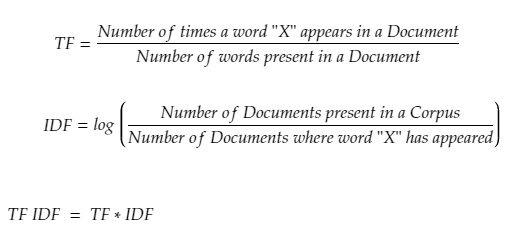
\includegraphics[scale=0.9]{tf-idf-formula.PNG}\\
    \textbf{Fig.1: Fórmulas para calcular TF-IDF}
    \end{center}
\end{frame}
\begin{frame}
    \frametitle{Anexos}
    \begin{center}
    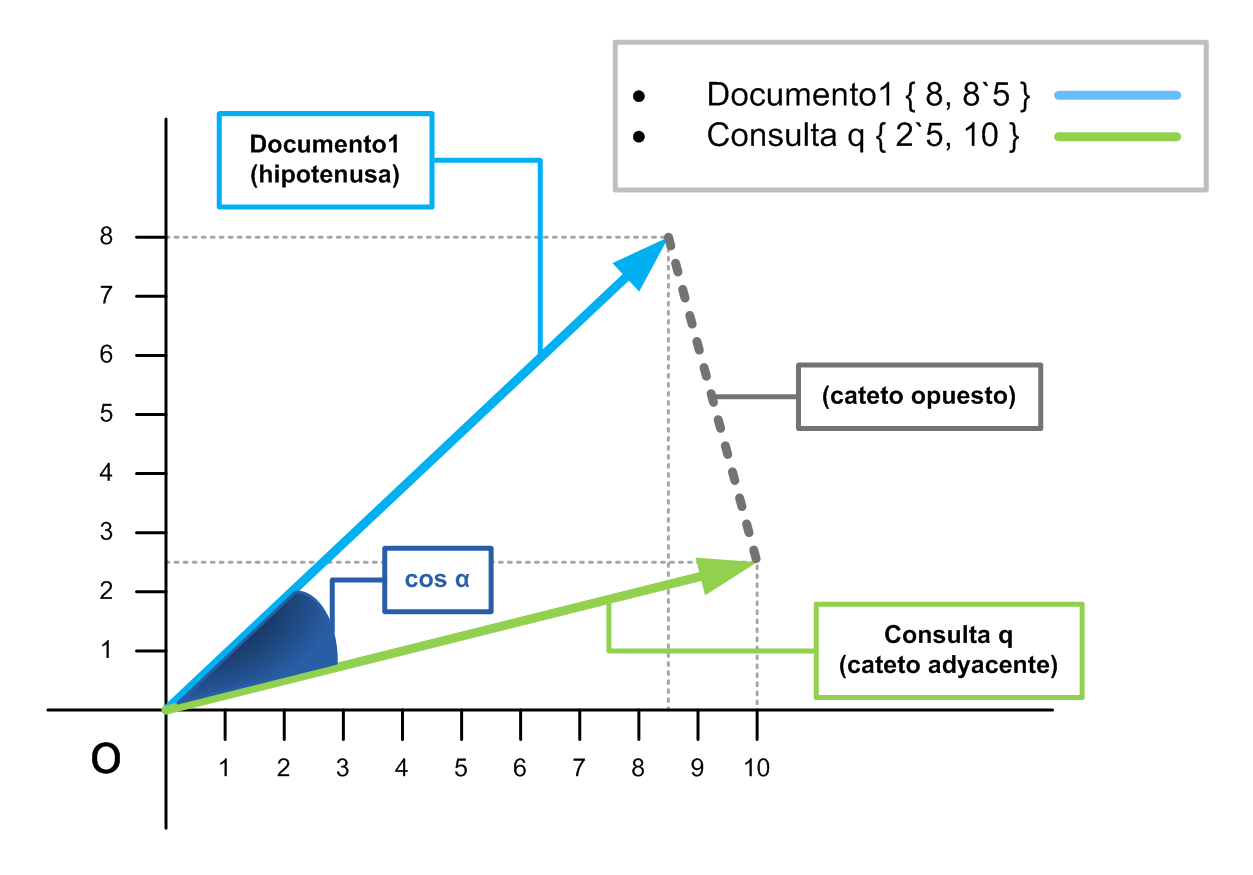
\includegraphics[scale=0.9]{figura12_vectorial.png}\\
    \textbf{Fig.2: Representación geométrica de la similitud de cosenos}
    \end{center}
\end{frame}
\begin{frame}
    \frametitle{Anexos}
    \begin{center}
    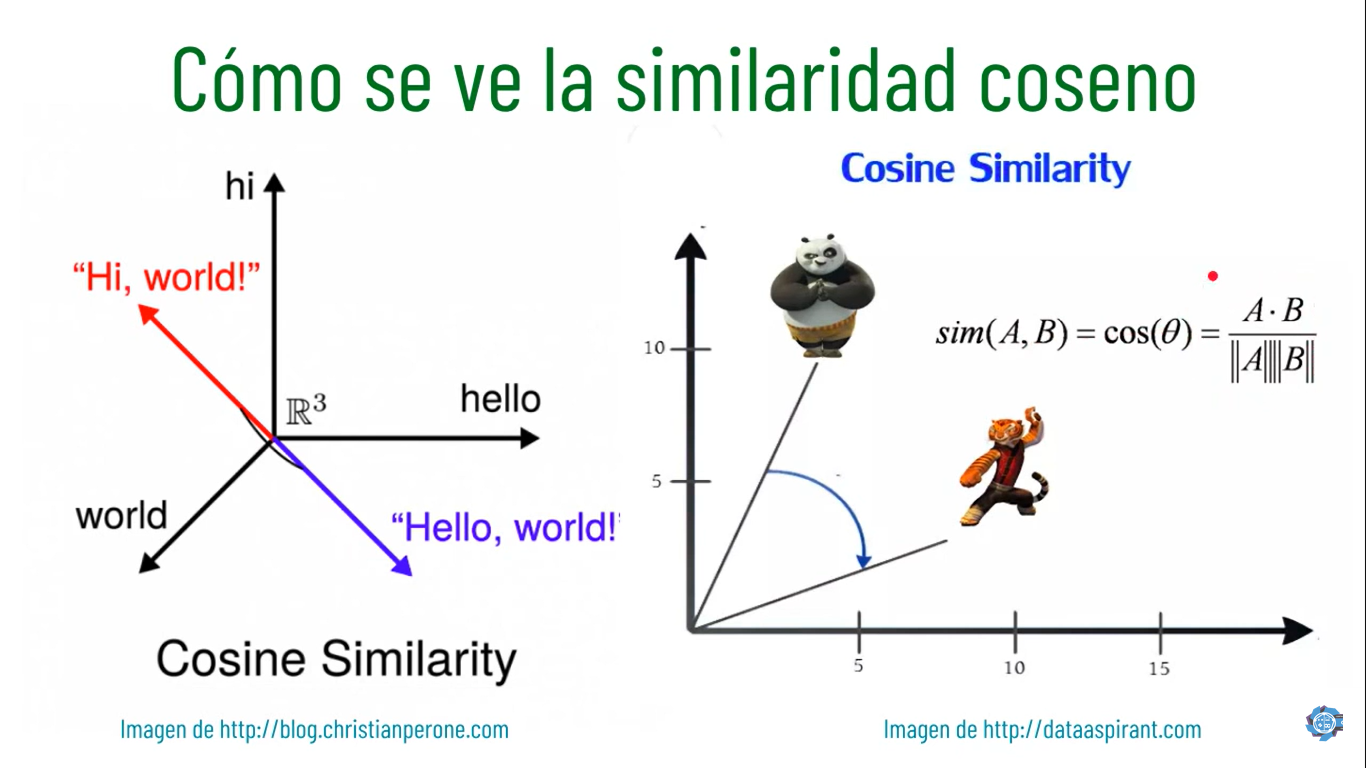
\includegraphics[width=12cm]{Sim Cos.png}\\
    \textbf{Fig.3: Fórmula Similitud de cosenos}
    \end{center}
\end{frame}
    \end{document}